% !TeX root = ../main.tex
% Add the above to each chapter to make compiling the PDF easier in some editors.

\chapter{Evaluation}\label{chapter:evaluation}
We evaluate our approach by first assessing the dice score between the each input tumor $\in P$ and the returned best-match. 
Then, we create a deterministic reference ranking:
Each of the 63 real tumors in $P$ is compared to 50,000\todo{50k?} synthetic tumors from $S$. The resulting dice scores for both segmentations and the combined values are ranked in 3 lists, yielding the rankings $R^{T1Gd}$, $R^{FLAIR}$ and $R^{Combined}$.\\
Based on these dice scores and rankings, we assess in \autoref{quantitative_eval} the baseline as well as the down sampling and compressions methods.
%by checking if the best mach of the optimization method is present in the best 1, 5 and 15 of the ground truth rankings.
In \autoref{qualitative_eval} we evaluate the quality of the baseline and its optimizations by examining results for selected tumors.
Finally, we investigated the embedding of our approach in the learn-morph-infer pipeline.
%- intro about different metrics: best match presence, partner index
%- evaluate compression techniques, lastly in the context of the entire pipeline eval baseline and compression techniques
%\section{Down Sampling}
%\section{Compression}
%- intro: encoded both $S$ and $P$ with the
\section{Quantitative Evaluation}\label{quantitative_eval}

\subsection{Baseline}
Before testing the different optimizations, we have to first assess the quality of the baseline results. 
In \autoref{fig_input_best_match_dice_scores} we examine the dice scores between the best match from the iterative baseline and the input tumor.
This analysis suggests that the current dataset is not sufficient to extract a close match for real tumors. 
We still investigate this approach further, since the underlying Dataset can be improved, e.g. by adding more data points.
A bigger Dataset would however inevitably worsen the runtime issue and therefore benefit even more from potential optimizations.
\begin{figure}[htbp]
  \centering
  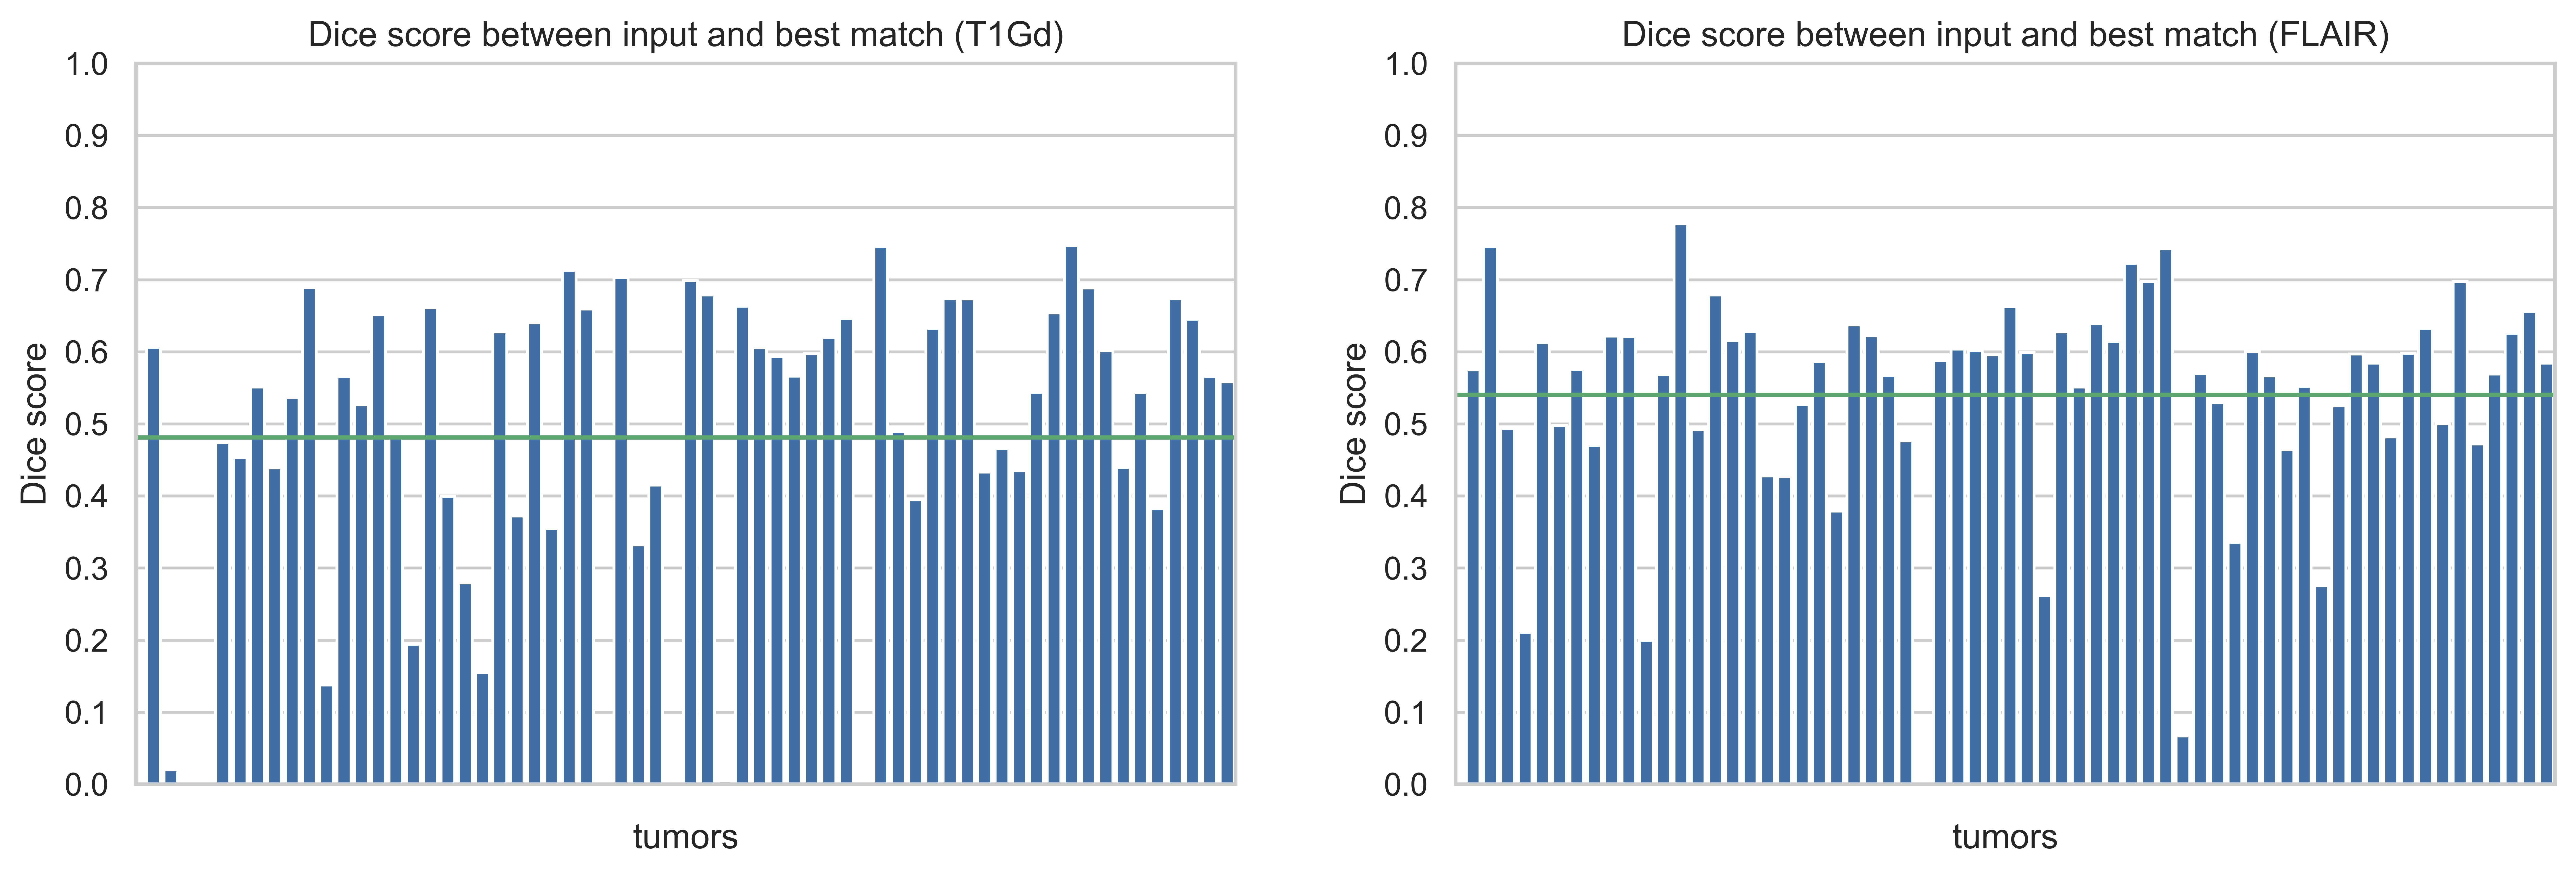
\includegraphics[width=450pt]{figures/input_best_match_dice_scores.png}
  \caption{
  Dice scores between the best match and real input tumors \todo{Check if input needs to be registered}
  }\label{fig_input_best_match_dice_scores}
\end{figure}
\FloatBarrier
\subsection{Optimizations}
In a theoretical transfer to clinical practice, our proposed query would return the best match of the comparison. 
In order to evaluate the quality of this best match, we check if the returned tumor is in the top 1, 5 and 15 results of the ground truth rankings $R^{T1Gd}$, $R^{FLAIR}$ and $R^{Combined}$.
\todo{mention other tried metrics, maybe move to trainging section to explain how values were chosen}
\subsubsection{Down sampling}
% best match presence table for t1gd, flair, combined
\subsubsection{Autoencoder}
% best match presence table for t1gd, flair, combined

\subsubsection{Variational Autoencoder}
% best match presence table for t1gd, flair, combined
\todo{print big baba table with all comparisons}
\section{Qualitative Evaluation}\label{qualitative_eval}
% choose a set of a few tumors taht will be used throughout the enxt subsubsections
% maybe use 1 chart for all, 2,3 cols for tumors -> orws are recosntructions (maybe just for t1c or both for 2, or table similar to kevins 
\subsection{Baseline}
% compare set of tumors with baseline results, visuals
\subsection{Optimizations}
\subsubsection{Down sampling}
% compare set of tumors with down sampling results, visuals
\subsubsection{Autoencoder}
% compare set of tumors with ae results, visuals
\subsubsection{Variational Autoencoder}
% compare set of tumors with vae results, visuals

\section{Performance in the pipeline context}
